\documentclass [bachelor,english,a4paper,11pt,oneside,webreferences,glossary,indextop,listoflistings,acronyms]{INSOthesis}
% change encoding in the document
%\inputencoding{utf8} % default
%\inputencoding{latin1} % for windows

\thesistitle{Peer to Peer collaborative editing based on a git repository}
%\thesisshorttitle{Shorttitle of the Thesis}
%\thesissubtitle{Optional Subtitle} % optional
\thesisdate{\today}

% all titles and designations have to be gender-related!
%\thesistype{Diplomarbeit}{Master's Thesis}
%\thesisdegree{Diplom-Ingenieurin}{Diplom-Ingenieurin}
\thesiscurriculum{Software \& Information Engineering}{Software \& Information Engineering} % your study
\thesisauthor{Stefan Gussner} % your name
\thesisauthoraddress{Margarethenstraße 30, 1040 Wien} % your address
\thesismatrikelno{01527253} % your registration number

% advisor
%\thesisauthorpreamble {Verfasser}
%\thesisadvisorpreamble {Betreuung}
% \thesisadvisorone {}
\thesisadvisortwo {Johann Grabner}
% \thesisadvisorthree {Vorname Nachname}

% Bibliographie file
\bibliography{bibliography/references}

\hypersetup{
  %colorlinks=false % enable and disable frames arround links
}

%%%%%%%%%%%%%%%%%%%%%%%%%%%%%%%%%%%%%%%%%%%%%
%
% Can be used to add additional informations
%
%%%%%%%%%%%%%%%%%%%%%%%%%%%%%%%%%%%%%%%%%%%%%
% \AfterTitlePages{}
% \AfterDeclaration{}
% \AfterAcknowledgements{}
% \AfterAbstract{}
% \AfterListOfFigures{}
% \AfterListOfTables{}
% \AfterAbbreviations{}
% \AfterBibliography{}

\renewcommand\afterchapternum{\hspace{1em}}
\begin{document}

\maketitle

\numberwithin{figure}{section}
\numberwithin{table}{section}

%%%%%%%%%%%%%%%%%%%%%%%%%%%%%%%%%%%%%%%%%
%%%   CONTENTS    %%%%%%%%%%%%%%%%%%%%%%%
%%%%%%%%%%%%%%%%%%%%%%%%%%%%%%%%%%%%%%%%%

%%%%%%%%%%%%%%%%%%%%%%%%%%%%%%%%%%%%%%%%%%%%%%%%%%%%%%%%%%%%%%%%%%%%%%%%
\chapter{Introduction}
\label{sec:introduction}
%%%%%%%%%%%%%%%%%%%%%%%%%%%%%%%%%%%%%%%%%%%%%%%%%%%%%%%%%%%%%%%%%%%%%%%%

%=======================================================================
\section{Problem Description}
%=======================================================================

When multiple people are working on solving a Problem it is not clear who is implementing which part. Current vcs systems conflict resolutions require manual conflict resolution if multiple people have modified the same file.
In order for a group to discuss a problem all the code has to be commited and pulled by everyone first. This introduces friction. In order to solve these and other problems real time collaborative editors have been created.
But current implementations of real time collaboration editors / editor plugins are unaware of the underlying version control system and therefore are based on the idea of just sharing files of a host mashine or a single source of truth file on a server instead of basing edit histories on versions of files known to the version control system anyway.

In state of the art collaborative code editors it is not possible for a user to easily see who made specific changes. Usually all the changes are bundled in one commit and the accountability is lost. In order to convert this concurrent model to a commit understood by Git it should be possible to stage changes by author. This approach might require more sophisticated logic than just interpreting changes as strings given that a command could be modified by two users and applying only half the changes as part of a commit could result in invalid syntax or semantic.

\section{Expected Results}

Enable real time collaboration on source code based on a Git\footnote{\href{https://git-scm.com/}{https://git-scm.com/}} project by
continuous tracking of code changes synchronizing over peer to peer connection.
Lowering overhead of splitting tasks by enabling everyone see what other people are working on. Allowing discussions about source code that has not yet been commited.
Changes should be commitable by author. In order to be able to compile sourcecode, changes of other people can be toggled off.
Using Git as a base enables opportunistic real time collaboration. In other words if a connection is possible changes will be propagated  to other people working on the same branch. If not the changes will be sent when a connection is available. \cite{AlwisSillito:2009:centralToDecentralVCS},\cite{6188603} Therefore it should be analog to the benefits of moving to a decentralized vcs.

%=======================================================================
\section{Motivation}
%=======================================================================

Current implementations of real time collaboration tools are not designed with version control systems in mind.

Transforming real time collaborative edits into regular Git commits by author will reduce a lot of friction in the adoption for real time collaboration software. Using a peer to peer solution with the ability to deal with disconnect events using information already known to the version control system will drasticly increase the ease of use. Ideally a user will not even have to think about using the extension.
%%%%%%%%%%%%%%%%%%%%%%%%%%%%%%%%%%%%%%%%%%%%%%%%%%%%%%%%%%%%%%%%%%%%%%%%
\chapter{Fundamentals}
\label{sec:fundamentals}
%%%%%%%%%%%%%%%%%%%%%%%%%%%%%%%%%%%%%%%%%%%%%%%%%%%%%%%%%%%%%%%%%%%%%%%%

%=======================================================================
\section{State of the Art}
\label{sec:stateoftheart}
%=======================================================================

This section describes and discusses current state of the art tools for real time collaboration.

\subsection{Teletype for Atom}
Teletype for Atom\footnote{https://github.com/atom/teletype/issues/211} is a Project enabling editing files peer to peer. It is based on 	\cite{Oster:2006:DataconsistencyforP2Pcollaborativeediting} \cite{YuWeihai:2014} \cite{BriotUrsoShapiro:2016:HighResponsivenessGroupEditing}.
With Teletype it is possible to edit files currently opened by the "host". The files are only persisted on the "host" not on all peers.\footnote{https://teletype.atom.io/}
Therefore disconnecting from the network cuts off the editing workflow. It is not possible to access all the files in a project unless they are opened by the host. 
\subsection{CoVim}
CoVim\cite{ChoNgSun:2017:CoVim:Incorporatingreal-timecollaborationcapabilitiesintocomprehensivetexteditors} uses Operational Transforms just like Teletype for Atom. But uses a different method of detecting state changes. Instead of observing user interactions it observes changes to files and generates Operational Transforms from diffing states.
\subsection{TouchDevelop}
TouchDevelop\footnote{https://www.touchdevelop.com} is an experimental web based editor. It enables real time collaboration by merging ASTs. The paper claims "Indeed, we claim that this approach is generalizable to a
general-purpose language, as long as the editor can parse the
program being edited and transparently tag AST nodes with
an identifier. Naturally, this requires non-trivial support from
the editor".\cite{ProtzenkoBurckhardtMoskalMcClurg:2015:Implementingreal-timecollaborationinTouchDevelopusingASTmerges} The AST translation would have to be implemented for every programming language supported. Additionally the transformation from AST to text might not guarantee the same code just the same AST which could lead to confusion for developers. 
\subsection{CodeR}
CodeR\cite{KurniawanSoesantoWijaya:2015:CodeR:Real-timeCodeEditorApplicationforCollaborativeProgramming} is a Web IDE with built in chat for the programming languages C, C++ and JAVA. 
\subsection{Visual Studio Live Share}
Visual Studio Live Share\footnote{https://visualstudio.microsoft.com/de/services/live-share/}  is a plugin for Visual Studio Code and Visual Studio that enables sharing all files of a project loaded in the editor with someone else. In addition to that it enables sharing debugging sessions and ports opened by debugging sessions are forwarded to clients. As with Teletype for Atom files are only persisted on the "host"  
\subsection{Multihack-Brackets}
Multihack-Brackets\footnote{https://github.com/multihack/multihack-brackets} is a plugin for the Brackets editor. It enables sharing an entire folder structure. It requires a server. As of 13.3.2019 it is not possible to verify performance or functionality since joining a session just crashes the brackets editor. 
\subsection{Codeshare}
Codeshare\footnote{https://codeshare.io} is a web based collaborative editor. It is designed for interviews. The editor window offers syntax highlighting for a broad range of programming languages. One shared room always only contains a single file. 
\subsection{Summary}
As described in \ref{tab:sota} current solutions are mostly implemented as extensions to code editors. Only codeshare is web based because it is based around the use-case of doing interviews. Overall none of the current solutions have any considerations for dealing with an underlying version control system of a project.

\begin{table}
	\centering
	\begin{tabular}{| >{\bfseries}l | l | l | l | l | }
		\hline
			\rowcolor{orange} \bfseries Tool & \bfseries Type & \bfseries Location & \bfseries Shared Content \\
		\hline
		\hline
			Teletype for Atom & Extension & Host & Individual Files \\\hline
			Visual Studio Live Share & Extension & Host & Project Folder \\\hline
			Multihack Brackets & Extension &  Distributed? & Project Folder \\\hline
			Codeshare & Web application & Server & Single File \\
		\hline
	\end{tabular}
	\caption{Overview state of the art}
	\label{tab:sota}
\end{table}

\section{CRDT}
In order to update shared objects stored at different sites a "commutative replicated data type" or CRDT is proposed by \cite{PreguicaMarquesShapiroLetia:2009}. The idea is to design the underlying representation or data structure of edits to a document such that operations are commutative and therefore automatically converge at every copy of the document.
But there is a problem with this approach. If there are concurrent insertions at the same position of a document, a global order for the conflicting information has to be established. \cite{PreguicaMarquesShapiroLetia:2009},\cite{Oster:2006:DataconsistencyforP2Pcollaborativeediting} have a solution to this problem: every site gets a unique siteID and a logical clock or counter. Concurrent inserts are then ordered either by the counter (smaller counter first) or if the counters are identical by the siteID.

\section{Code Review}

Companies like Google and Microsoft use a process called "code review" to validate changes. The basic idea is that before merging a code modification onto master, it is reviewed by someone else. This keeps code quality stable and educates developers.\cite{SadowskiSoederbergChurchSipkoBacchelli:2018:Moderncodereview:acasestudyatgoogle} This thesis aims to support these workflows while enhancing the developer experience. 

"Another thing we focused on was performance. For that
reason, even today CodeFlow remains a tool that works
client-side, meaning you can download your change first
and then interact with it, which makes switching between
files and different regions very, very fast."\cite{CzerwonkaGreilerBirdPanjerCoatta:2018:CodeFlow:ImprovingtheCodeReviewProcessatMicrosoft} Therefore another important goal for this thesis is to deliver an experience that works client side and keeps working when disconnecting and reconnecting to networks.
\chapter{Methodological Approach}

First a state of the art analysis will be conducted. This analysis will look into currently available open-source and commercial products for real time collaboration. 
Additionally the current literature related to real time collaboration will be studied.
The papers mentioned in open source projects will be used as a starting point for forwards and backwards literature analysis.


The following list of publishers will be used as sources of literature: ACM Digital Library\footnote{\href{https://dl.acm.org/}{https://dl.acm.org/}}, IEEE Xplore Digital Library\footnote{\href{https://ieeexplore.ieee.org/}{https://ieeexplore.ieee.org/}}, SpringerLink\footnote{\href{https://link.springer.com/}{https://link.springer.com/}}, and ScienceDirect\footnote{\href{https://www.sciencedirect.com/}{https://www.sciencedirect.com/}}. Google Scholar\footnote{\href{https://scholar.google.com/}{https://scholar.google.com/}} will be used as an additional search engine. Papers that are not published by the previously mentioned publishers will only be used in exceptional cases and after consultation with the supervising assistant.


The literature survey will be continuously documented in the following format:

\begin{lstlisting}
	<date>: <search query>
		<publisher>
			<paper title>
	<search query> := one of the following:
\end{lstlisting}

\begin{itemize}
    \item search terms
    \item conference
    \item forward/backward search paper title
    \item authors of specific papers 
\end{itemize}
If multiple searches occur on the same date, the date has to be included again for every search query.

Based on problems mentioned in papers and issues of projects from the state of the art analysis, requirements for the extension will be defined.
These requirements will be user centered.
Functional as well as non functional aspects such as performance will be defined as requirements.

Use-cases for the extension will also be defined. These use-cases directly related to editing source code will have defined number of users as well as file sizes in order to be verifiable. 
Every use-case includes at least the following information:
\begin{itemize}
    \item Actor (the steakholder)
    \item System (the software the actor is interacting with)
    \item Action (the goal of the actor)
\end{itemize}
A VS Code\footnote{\href{https://code.visualstudio.com/}{https://code.visualstudio.com/}} extension better suited to accomodate the identified use-cases will be implemented.
The extension will meet the following requirements:
\begin{itemize}
    \item The extension will target VS Code 1.32 or newer and will be written in node JS
    \item Automated testing will be used wherever possible and meaningful.
    \item The source code will be commented and well documented.
\end{itemize}
The thesis will be written in parallel with the development of the extension. Git will be used as a version control system for the thesis as well as the extension.

The solution will be evalutated by comparing the extension and the state of the art tools in terms of suitability for the specified use-cases. 
The evaluation will be based on the amount of time required to fulfill a specific use-case.
Furthermore, any limitations compared to state of the art solutions will be documented.
\chapter{Requirements}

\section{Share the entire project structure}

Every user should be able to see all changes to the project.
Based on this Issue and the discussion "Current implementation only shares current project. It would be more useful if I could share the whole project so two persons can work on different files."\footnote{\href{https://github.com/atom/teletype/issues/211}{https://github.com/atom/teletype/issues/211}} being able to edit the entire project structure is a very important feature.

\section{Only display changes in the same Git branch}

Given that a lot of developers are using prototype branches and a significant number are usign feature branches Git branches are a good indication that a specific problem is being worked on.\cite{PhillipsSillitoWalker:2011:Branching_and_merging} Therefore only displaying cuncurrent edits on the same edit removes noise of unrelated edits.

\section{Stage changes by author}

Synchronizing changes to all developers introduces a problem:
"[\dots]This means that git only becomes a way to have a backup as all the work is done using P2P! [\dots]"\footnote{\href{https://github.com/atom/teletype/issues/211\#issuecomment-478306010}{https://github.com/atom/teletype/issues/211\#issuecomment-478306010}}
Possibly unrelated modicications would be bundled into huge commits. In order to mitigate this, changes should be stageable by author.

\section{Respect .gitignore}

Files explicitly excluded from the version control system via the .gitignore file\footnote{\href{https://git-scm.com/docs/gitignore}{https://git-scm.com/docs/gitignore}} should not be synchronized with other client as these files might contain automatically generated files that depend on the local system configuration or contain sensitive information.

\section{Performance}

Although "VS Code aims to deliver a stable and performant editor to end users, and misbehaving extensions should not impact the user experience. The Extension Host in VS Code prevents extensions from:
\begin{itemize}
    \item Impacting startup performance
    \item Slowing down UI operations
    \item Modifying the UI
\end{itemize}"\footnote{\href{https://code.visualstudio.com/api/advanced-topics/extension-host}{https://code.visualstudio.com/api/advanced-topics/extension-host}}
Performance of the extension should be good enough that typing on two computers with one hand each should be possible without introducing errors or noticable delay if both computers are connected to the same network via ethernet.

Scenario: A person is sitting in front of two computers both with vscode and the extension open. The left hand is on the keyboard of the first computer, the right hand on the keyboard of the second computer. The person should be able to type a sentence without errors being introduced by delays in change synchronization.


\chapter{User stories}

As a programmer I want to have access the entire project structure when using a code editor.

As a programmer I want clean seperation between branches and do not want to see changes to other branches when using a version control system.

As a programmer I want to be able to stage changes that I made to Git.

As a project manager I want to see who made a specific modification to a project in the version control system.

As a programmer I do not want to configure a second version control system when I already provided this information to Git.

As a programmer I do not want files covered by my .gitignore configuration to be shared with others.

As a programmer I want to be able to edit files with up to 4 people at a time. A file can have up to 30.000 characters.

\chapter{Scenarios}
Ih this section multiple scenarios are derived from the user stories.

\section{Scenario 1}
Person A and B are working on an Node.js Express project together. Person A is working on branch Ba, person B is working on Branch Bb.
Person A has edited the file /app.js (paths are described as absolute from the project root) as well as the file /routes/account.js on Ba.
Person B has edited the file /app.js as well as the file /routes/main.js on Bb.
Person A encounters unexpected behaviour of his code. He requests help from person B.
Neither persons A nor B want to commit their changes at this point.
Person B uses the VS Code Command Palette and chooses the option "Procurrently: Checkout Branch" and chooses branch Ba.
Person B now sees only the modifications in /app.js and /routes/accounts.js from branch Ba.
Upon discovering the problem in the sourcecode, person B modifies /routes/account.js to solve the problem.
Person A can see the the changes in real time.
Person B once again opens the VS Code Command Palette and chooses the option "Procurrently: Checkout Branch" and chooses branch Bb.
Person B now sees the modifications in /app.js and /routes/main.js on Branch Bb and can continue working on his task.

\section{Scenario 2}
Person A and B are working on an Node.js Express project together. Both of them are working on branch master in the /app.js file.
Person A is modifying and testing a new feature while person B is working on setting new HTTP caching headers for the Express app.
This is interfering with the test of person A. Person A opens the VS Code Command Palette and chooses the option "Procurrently: Toggle remote changes".
All the modifications of B are reverted in the documents of person A.
During that person B can still see the modifications of person A which helps person B to determine the correct caching headers for the different routes.
Person As laptop disconnects from the network. Therefore person B can no longer recieve real time updates from person A.
Person As laptop reboots unexpectedly. Once the laptop is booted up again, person A opens VS Code and can continue to work where he left off.
Person A now wants to know about the progress of person B and turns on remote changes. Person A can see all the changes of person B until person A disconnected from the network. Person A disables remote changes again and continues to work on his new feature.
Later on person Bs laptop reconnects to the network and person B can recieve all the modifications person B missed.
Once person A is happy with the implementation of the new feature, he wants to test the caching behaviour himself to make sure person B has understood his code correctly.
Person A opens the VS Code Command Palette and chooses the option "Procurrently: Toggle remote changes".
Person A now sees all the modifications of person B again including the modifications B made while person A had disabled the remote changes.
\chapter{Implementation}

This chapter describes the implementation details of Procurrently, the extension for VS Code. It gives an overview of the Git library, that needed to be developed sinve other available solutions would not work inside a VS Code extension context as well as used VS Code APIs. Additionally the data structure and change handling by the extension are described.

\section{Git}

Git provides useful information about the current project, the developer is working on, such as:
\begin{itemize}
    \item The current branch (the problem being worked on)
    \item The root directory of the project (for path resolution across devices)
    \item The current version of a file (as a basis for collaborative edits)
    \item Information about the developer (the username)
\end{itemize}

Git stores this information in the ".git" directory in the root folder of the project.
The data is stored in a compressed format. In order to access the information, a small library using low level Git commands was implemented. 
A custom implementation was nessesary because the NodeGit\footnote{https://github.com/nodegit/nodegit} library would crashes VS Code as soon as the extension would import it.

The Git library provides a low level interface for interacting with a Git repository. It provides functions to find the Git directory for a given file (given the file is inside a Git repository) and retrieve information like the path of a file within the repository, information about the current commit, hash, branch, remote URL, username of the repository, versions of a file. This information is crucial for determining the version of a file that has been modified by the user and finding the identical file on the mashine of another user.

Additionally the Git library provides function to stage files for commit, commit changes and do a Git reset. The stage and commit functions are required in order to stage changes by author and commit them. The Git reset function is used to synchronize file contents to the version known to Git. This enables synchronizing the files without establishing base versions of files over the network first.

The Git library can invoke a callback function when the current state of a repository changes. This is the case if a different branch is checked out or the current commit changes due to the user commiting or a git pull. Because once the repository changes, the appropriate changes have to be applied to documents and only changes for the same repository state can be replayed.

\section{teletype-crdt}
\label{sec:teletypecrdt}

"The string-wise sequence CRDT powering peer-to-peer collaborative editing in Teletype for Atom."\footnote{https://github.com/atom/teletype-crdt}
This library will be used for tracking changes. It is written in JavaScript and currently does not include an API documentation.


Teletype-crdt provides the Document class. This class represents a shared document using a CRDT. In order to notify the document representation about a local change, the setTextInRange (see \autoref{lst:setTextInRange}) function can be used.

When a change from another instance of the document is recieved, the teletype-crdt document can be notified using the integrateOperations (see \autoref{lst:integrateOperations}) function. This function returns a set of TextUpdates, which are changes to the text of the document to match the operations.

Since the document turns every text change into an operation and operations contain information about the author, sometimes the effect of operations need to be determined. For example if staging changes by author. To do this, the undoOrRedoOperations function is used (see \autoref{lst:undoOrRedoOperations}). It returns a set of modifications for the file on disk equivalent to an undo of a set of operations. Which, if this function is not used otherwise translates to the mapping of operations to effects of operations described above.


\begin{lstlisting}[label={lst:setTextInRange}, caption=teletype-crdt setTextInRange]
setTextInRange(start: {row:Number, column:Number}, end: {row:Number, column:Number}, text: string, options?: any): [operation];
\end{lstlisting}

\begin{lstlisting}[label={lst:integrateOperations}, caption=teletype-crdt integrateOperations]
integrateOperations(operations: [operations]): {textUpdates:[textUpdate], markerUpdates:any};
\end{lstlisting}

\begin{lstlisting}[label={lst:undoOrRedoOperations}, caption=teletype-crdt undoOrRedoOperations]
undoOrRedoOperations(operationsToUndo: [operation]): any;
\end{lstlisting}

\subsection{Git and teletype-crdt}
As a basis for the edit history  the current Git commit in the current branch will be used. Teletype-crdt uses numeric siteIds to identify changes by author. The current Git commit is imported as edited by siteId 1 upon discovering the file. By doing this, all clients have an initial shared state based on the current version of the file known to Git.

\section{VS Code Extension API}

VS Code runs extension in a seperate process and provides an asynchronous Javascript API.
The examples provided in the vscode-extension-samples repository\footnote{https://github.com/Microsoft/vscode-extension-samples} are mostly written in Typescript\footnote{https://www.typescriptlang.org/} and all the Interfaces have type definitions for Typescript.
Therefore the Extension will use Typescript as well.

\subsection{Used API Functions}

The VS Code API provides a set of asynchronous functions that return Promises. Promises have been added in ECMAScript 6 and provide a standardised way of handling asynchronous code in ECMAScript.\cite{Madsen:2017:MRJ:3152284.3133910} ECMAScript is the standard for the JavaScript language.

Procurrently mainly uses the onDidChangeTextDocument (see \autoref{lst:onDidChangeTextDocument}) and the applyEdit (see \autoref{lst:applyEdit}) function. 

Using the onDidChangeTextDocument function (see \autoref{lst:onDidChangeTextDocument}), a callback function is invoked whenever a text document is changed.\footnote{https://code.visualstudio.com/api/references/vscode-api\#workspace} This callback function converts the event provided by VS Code to a teletype-crdt operation using using the setTextInRange function (see \autoref{sec:teletypecrdt}) and sends the resulting operation to all other peers.

Other peers subsequently use the applyEdit function (see \autoref{lst:applyEdit}) to apply the TextUpdates from the integrateOperations function (see \autoref{sec:teletypecrdt}) to the document on disk.

\begin{lstlisting}[label={lst:onDidChangeTextDocument}, caption=VS Code API onDidChangeTextDocument]
vscode.workspace.onDidChangeTextDocument()
\end{lstlisting}

\begin{lstlisting}[label={lst:onDidOpenTextDocument}, caption=VS Code API onDidOpenTextDocument]
vscode.workspace.onDidOpenTextDocument()
\end{lstlisting}

\begin{lstlisting}[label={lst:applyEdit}, caption=VS Code API applyEdit]
vscode.workspace.applyEdit(edit)
\end{lstlisting}

\autoref{lst:applyEdit} returns a promise which resolves when the change has been added to the text document.
An edit is given by a document, the line and column of start and end of the edit in that document and the new text to be inserted there.
If text is added or removed within a line, the columns of the text change after the edit has been applied (when the promise resolves). If another edit is applied before the promise resolved, the indices of the text might have not been changed yet and therefore at a different position than expected. VS Codes WorkspaceEdit supports grouping change operations together. But change operations are not treated as happening all at a time so if for example the text "123" was typed the teletype-crdt library would essentially output Line 1 Char 1 to Line 1 Char 1 changed to "1", Line 1 Char 2 to Line 2 Char 2 changed to "2" and so on. This is kind of expected behaviour so far but VS Code's WorkspaceEdit treats this as independent operations and if there was text after the insertion the changes would not be inserted as one block but interlaced with the previous text. 

In order to avoid this race condition all changes to a file have to be carried out sequentially. This is not noticable when changes by regular typing are integrated into the local document. But when the multiple cursors\footnote{https://code.visualstudio.com/docs/getstarted/tips-and-tricks\#\_editing-hacks} are used the change integration can slow down noticably. In order to support multiple cursors the changes are sorted by column in decending order to prevent shifting indices. (See \autoref{lst:sort_changes})
\begin{lstlisting}[label={lst:sort_changes}, caption=Sorting Changes by Column to Prevent Index Shifting]
textUpdates.sort((a, b) => b.oldStart.column - a.oldStart.column)
\end{lstlisting}

\subsection{Tree View}

In order to stage changes by author, a Tree View listing the Authors, who made changes, was created.
The container for a Tree View needs to be defined in the package.json file. \autoref{fig:treeview}

\begin{minipage}{\linewidth}
\begin{lstlisting}[label={lst:contributes_treeview_activitybar}, caption=Tree View Activitybar]
"contributes": {
    "viewsContainers": {
        "activitybar": [
            {
                "id": "change-explorer",
                "title": "Change Explorer",
                "icon": "media/icon.svg"
            }
        ]
    }
    [...]
}
\end{lstlisting}
\end{minipage}

First an entry in the activity bar has to be declared in the viewsContainers section (See \autoref{lst:contributes_treeview_activitybar}). It defines the icon as well as the hover text (called title) of the tab in the activity bar.

\begin{lstlisting}[label={lst:contributes_treeview_view}, caption=Tree View Pannel Definition]
"contributes": {
    [...]
    "views": {
        "change-explorer": [
            {
                "id": "contributors",
                "name": "Contributors"
            }
        ]
    }
}
\end{lstlisting}

\begin{figure}[hb]
    \centering
    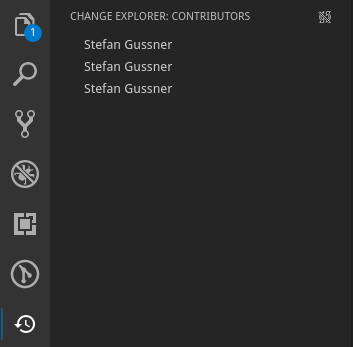
\includegraphics{figures/screenshots/treeview.png}
    \caption{Tree view}
    \label{fig:treeview}
\end{figure}

Additionally the view has to be declared.\autoref{lst:contributes_treeview_view} This defines the heading for the Tree View.

\begin{lstlisting}[label={lst:contributes_treeview_register}, caption=Define Tree View Data Provider]
const treeview = new ContributorsTreeView(crdt.getUsers);
vscode.window.registerTreeDataProvider('contributors', treeview);
\end{lstlisting}

To populate the Tree View with data, a TreeDataProvider has to be registered to the view id. (See \autoref{lst:contributes_treeview_register})
The TreeDataProvider interface defines functions that return all items for the Tree View as well as refresh the content of the Tree View.

\section{Data Model}

\begin{lstlisting}[label={lst:datamodel_declarations}, caption=Data Model Declarations]
const documents = new Map<string, { document: Document, metaData: { commit: string, branch: string, repo: string, file: string, users: Map<Number, string> } }>();
/** remote repository to path mapping */
const localPaths = new Map<string, string>();
/** The current branch for a file */
const branches = new Map<string, string>();
\end{lstlisting}

All the data is stored in a map called documents.(See \autoref{lst:datamodel_declarations})
It's key is composed of the filename and a specifier composed from the commit, branch and remote/origin repository URL.

In order to keep track of the current branch and head commit of files, the branches map contains the identifier for a file by filepath.

The localPaths map contains mappings from remote/origin urls to local Git directory locations.
This enables keeping track of files across different projects.


The documents map values contain

\subsection{The Document Object}

The document object has two properties

\begin{itemize}
    \item document
    \item metaData
\end{itemize}

The document property points to an instalce of the document class provided by teletype-crdt.

The metaData property contains the relevant information from Git about the document:
\begin{itemize}
    \item branch
    \item commit
    \item repo
    \item file
    \item users
\end{itemize}

The users property contains a map with the teletype-crdt siteId as a key and the Git username as a value.
This information is required to display usersnames in the staging Tree View.

\section{Reacting to Local Changes}
If a file has not yet been accessed, it has to be registered. This establishes the current version of the file known to Git. Additionally The localPaths map is updated with the repository remote origin URL as the key and the location of the git repository on disk as the value. This will later be used for incoming changes.

In order to process a local change, provided by the onDidChangeTextDocument API call, the extension checks, if the change has been added by a remote client. This is necessary because the VS Code API does not differentiate between changes by the user and changes by extensions. (See \autoref{lst:localchange_check_known}) Otherwise changes are duplicated endlessly because every remote change is propagated back to all other clients as a new change.

\begin{lstlisting}[label={lst:localchange_check_known}, caption=Is This Change Already Known to The Data Model? ]
const objects = ['start', 'end'];
const props = ['line', 'character'];

//check if this change has just been added by remote
const knownChanges = currentChanges
    .filter(c => 
        objects.map(o => 
            props.map(p => 
                c[o][p] == change.range[o][p])) 
        && c.text == change.text 
        && c.filepath == e.document.fileName);
if (knownChanges.length > 0) {
    //remove from known changes
    currentChanges.splice(currentChanges.indexOf(knownChanges[0]));
}
\end{lstlisting}

To update the teletype-crdt document the setTextInRange function is used. It returns a list of operations. This list of operations is sent in a JSON object containing the metaData associated with the document. (See \autoref{lst:change_json})

\begin{lstlisting}[label={lst:change_json}, caption=Network Data Packet]
{
    "update": {
        "metaData": {
            "branch": "refs/heads/master",
            "commit": "05fc4663235f36ba054ea37fd7f92e9a5555edf2",
            "repo": "git@bitbucket.org:company/a_repository.git\n",
            "file": "/app.js",
            "users": {}
        },
        "operations": [
            {
                "type": "splice",
                "spliceId": {
                    "site": 2766400253437581,
                    "seq": 3
                },
                "insertion": {
                    "text": "a",
                    "leftDependencyId": {
                        "site": 0,
                        "seq": 0
                    },
                    "offsetInLeftDependency": {
                        "row": 0,
                        "column": 0
                    },
                    "rightDependencyId": {
                        "site": 2766400253437581,
                        "seq": 1
                    },
                    "offsetInRightDependency": {
                        "row": 0,
                        "column": 0
                    }
                }
            }
        ],
        "authors": [
            [
                2766400253437581,
                "Stefan Gussner"
            ]
        ]
    }
}
\end{lstlisting}

\section{Network Transport}

\subsection{Establishing the Peer To Peer Connections}
When the extension is activated, a to a bootstrap server is established. 
The peer sends the bootstrap server his ip as well as the port of the socket, the peer is listening on for incoming connections.
Upon recieving this information the bootstrap server responds with a list of ips and ports of all the other registered peers.
The peer then tries to connect to every peer in that list.

Once a connection is established, the peers exchange all the changes they know about.

\subsection{Handling Changes}
Every change is propergated to every node known to the peer. This approach is performant enough for small groups. To scale up to more clients, peers could intelligently only send changes to peers, who are currently on the same branch and peers could request operations from other peers when switching branches. Additionally changes could be propergated via a gossip based protocol.

\section{Handling Remote Changes}

Handling incoming changes has two main challanges:
\begin{itemize}
    \item concurrent changes
    \item finding files on disk
\end{itemize}

\subsection{Concurrent Changes}
\label{subsec:concurrentchanges}
Concurrent changes can introduce errors when adding them to a file. 
Given two changes on the same line one of the changes will have it's index changed by the other one.

To illustrate the problem consider this example:

The initial line consists of the string "12345".
Now peer A adds "g" after index 3 and peer B adds "c" after index 4
The local result for A is "123g45" and the local result for B is "1234c5".
The correct result for the changes would then be "123g4c5"
The crdt data type handles this concurrency problem and if the change from peer B is processed after the change from peer A the insert operation of B is adjusted from index 4 to 5.
But this assumes that all the changes are processed sequentially. If the order of insertions is not guaranteed the resulting string could turn into "123g45c" if the crdt document processes the changes in the order A -> B and the VS Code Edit is processed in the order B -> A.

To ensure consistency, the network layer waits for the change handling promise to resolve before processing the next change. This can be thought of as "pretending network changes have been delayed".
CRDTs such as atom-teletype are designed to handle delayed network packets. Therefore this ensures consistent change replication. \autoref{lst:promise_chain} ensures that incoming change packets are processed sequentially by building a promise chain.

\begin{lstlisting}[label={lst:promise_chain}, caption=Network Promise Chain]
this._currentEdit = this._currentEdit.then(() => {
    [...]
    return this._onremoteEdit(recieved.update);
    [...]
})
\end{lstlisting}

\subsection{Locating Files on Disk}

Given the information from the network locating the file the change corresponds to is not trivial.

First the appropriate Git repository has to be located.
This information can be looked up in the localPaths map.

If the file has not been accessed previously, the base version of the file has to be established.
By using the getCurrentFileVersion function of the Git library to retrieve the appropriate version from the Git repository to replay changes onto.

\subsection{Adding Changes to File}

If the file changed by the remote peer is currently checked out, the change has to be incorporated into it. Otherwise the change will just be saved to the atom-teletype document representation. (See \autoref{lst:add_change_to_local})

\begin{lstlisting}[label={lst:add_change_to_local}, caption=Adding Change to Local Document]
//only apply changes if on the same branch and remote changes visible
if (branches.get(filepath) == getSpecifier(metaData.commit, metaData.branch, metaData.repo) && remoteChangesVisible) {
    const doc = getLocalDocument(filepath).document;
    const textOperations = doc.integrateOperations(operations);
    try {
        await pendingRemoteChanges.then(() => applyEditToLocalDoc(filepath, textOperations));
    } catch (e) {
        console.error(e);
    }
} else {
    //save changes to other files
    getLocalDocument(filepath, metaData.commit, metaData.branch, metaData.repo).document.integrateOperations(operations);
}
\end{lstlisting}
%%%%%%%%%%%%%%%%%%%%%%%%%%%%%%%%%%%%%%%%%%%%%%%%%%%%%%%%%%%%%%%%%%%%%%%%
\chapter{Evaluation}
\label{sec:results}
%%%%%%%%%%%%%%%%%%%%%%%%%%%%%%%%%%%%%%%%%%%%%%%%%%%%%%%%%%%%%%%%%%%%%%%%

In this chapter Procurrently will be evaluated based on the scenarios and compared to existing tools.
Furthermore, limitations compared to other tools will be described.

\section{Evaluating Scenarios}

Procurrently was evaluated using the scenarios described in \autoref{sec:scenarios}.
These were tested on a real git repository containing 600 files. One of the files most commonly used in testing was app.js containing over 7000 characters or about 200 lines. The test was run on two MacBook Pros using an 802.11ac Wi-Fi connection.
The bootstrap server was run on one of the MacBooks. The IP for the bootstrap server was configured before starting the test using the VS Code settings menu. 

\subsection{Scenario 1}

The branches used in the test were "bug-hunt" and "buildsystem-test". On branch bug-hunt the files /app.js (see \autoref{fig:1appjs_on_bughunt}) and /routes/account.js (see \autoref{fig:1account_on_bughunt}) were modified by inserting comments. The configured username was "Stefan Gussner". 
After that on branch "buildsystem-test" the files /app.js and /routes/index.js were modified by inserting comments. The configured username was "Michael".


\begin{figure}
    \centering
    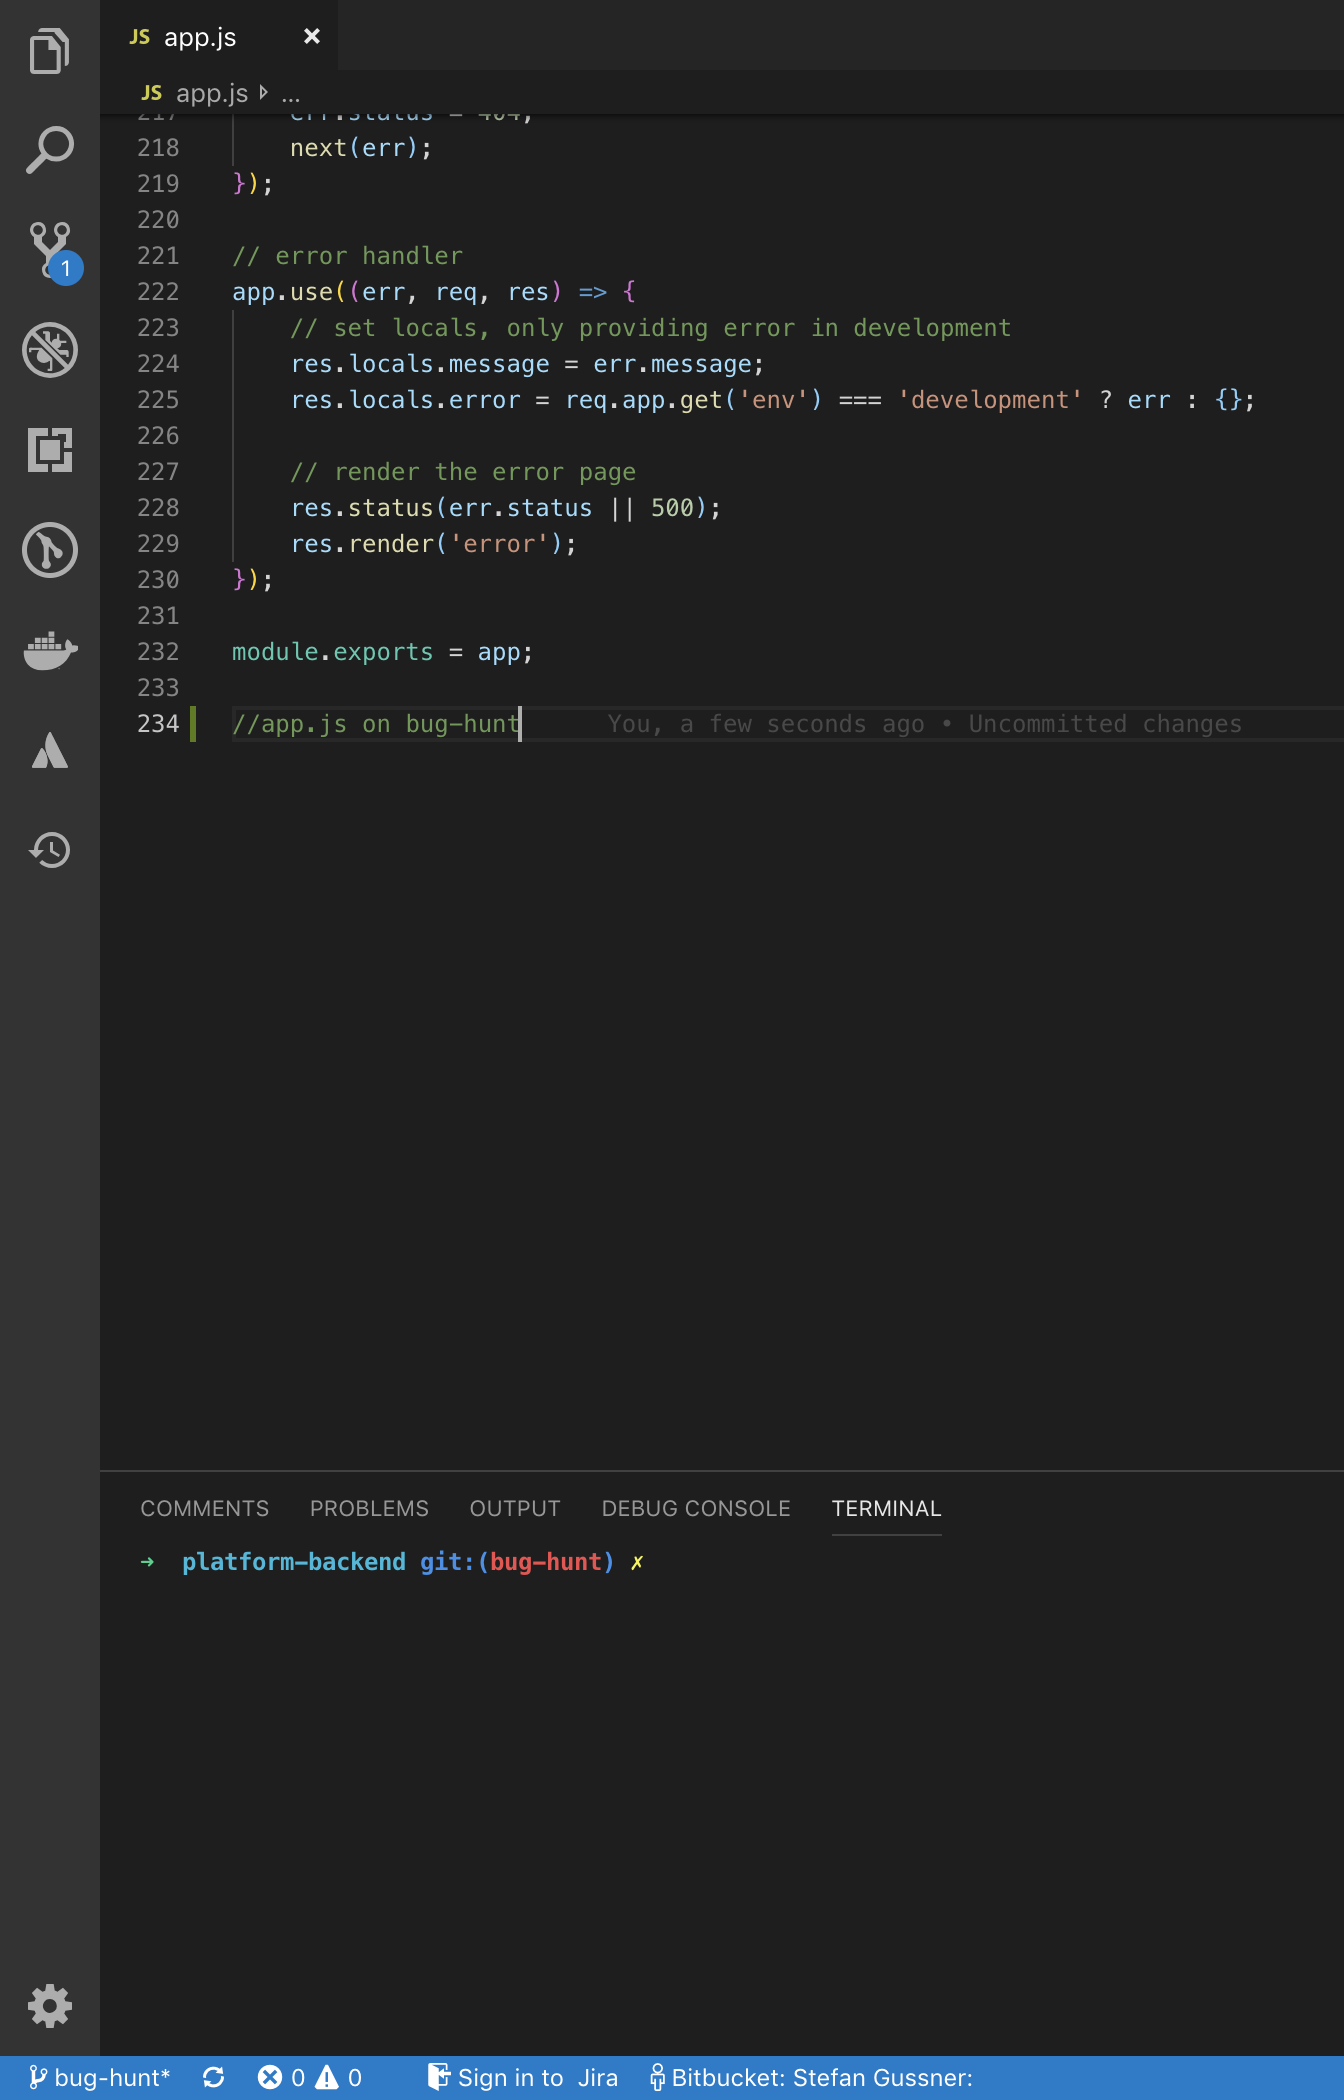
\includegraphics[width=1\linewidth]{figures/screenshots/scenarios/1appjs_on_bughunt.png}
    \caption{Scenario 1: Branch bug-hunt initial modifications app.js}
    \label{fig:1appjs_on_bughunt}
    \end{figure}
\begin{figure}
    \centering
    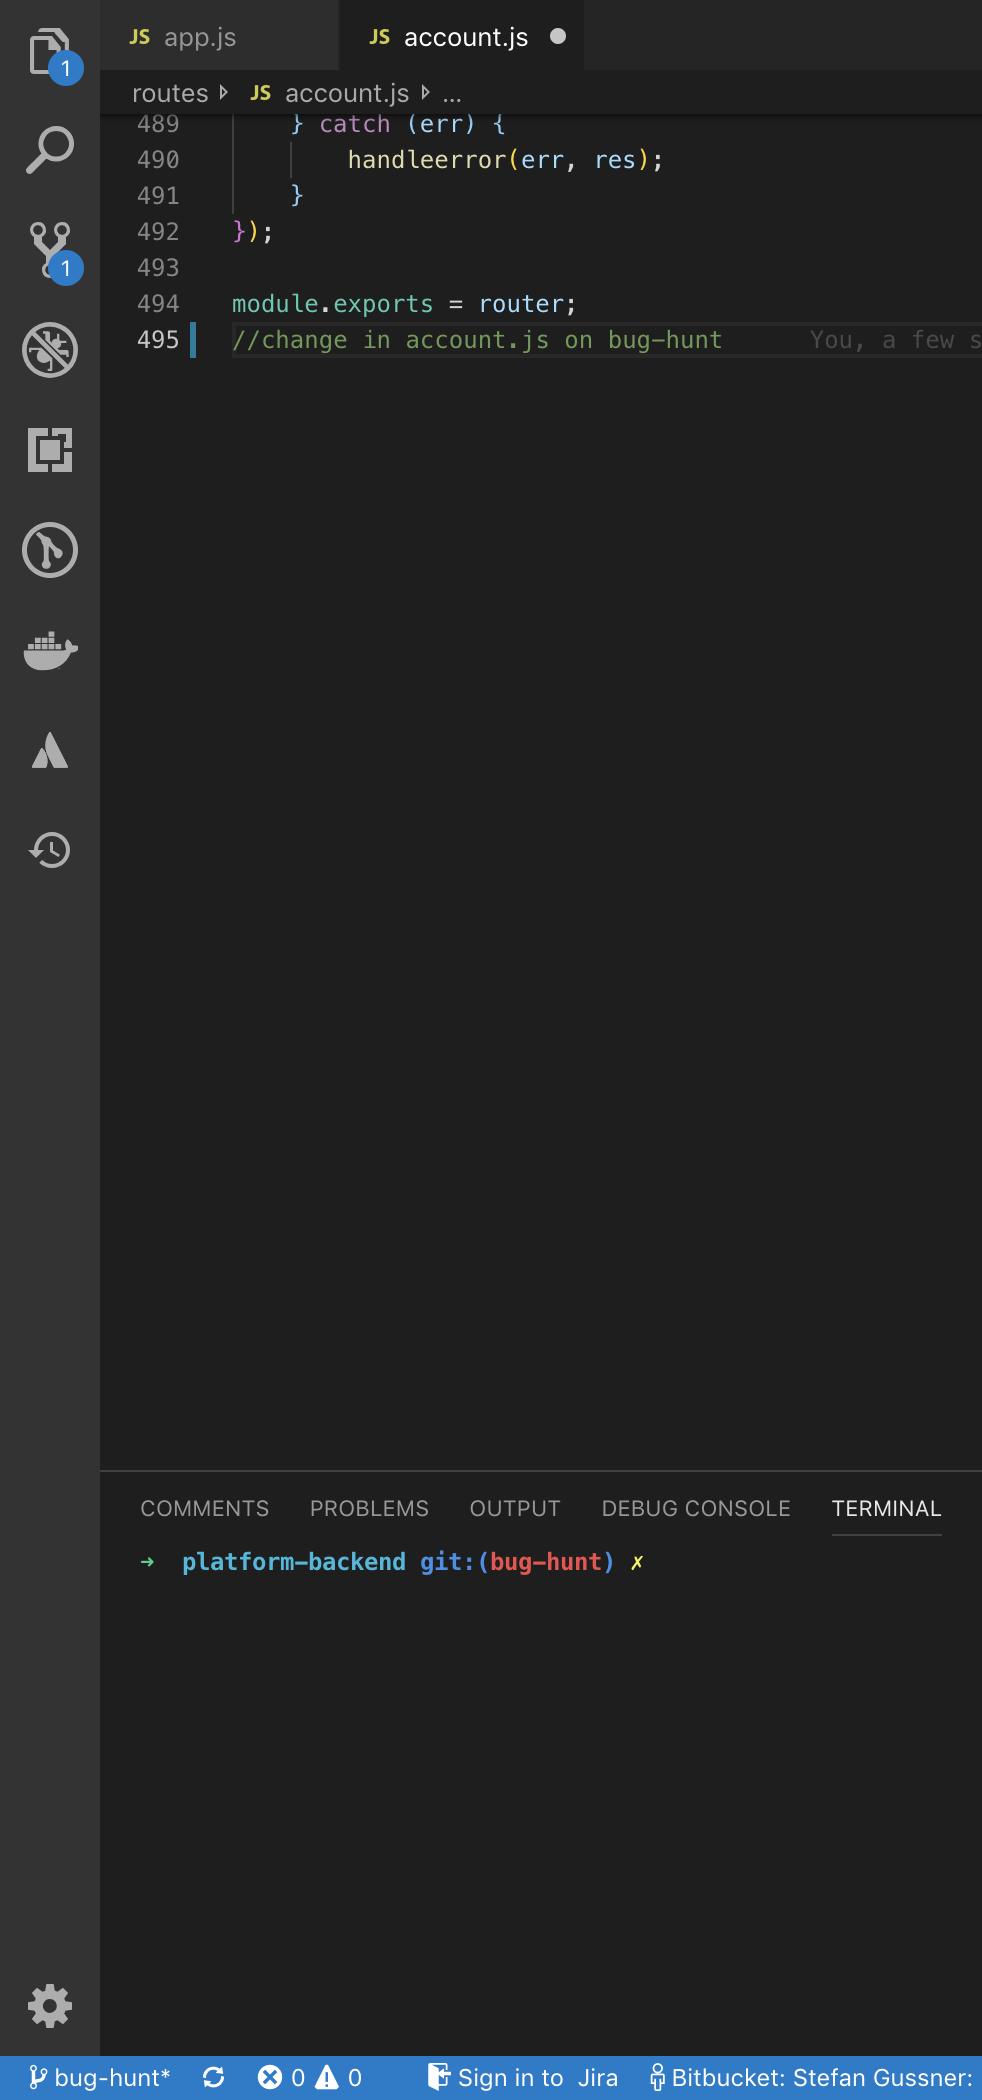
\includegraphics[width=1\linewidth]{figures/screenshots/scenarios/1accountjs_on_bughunt.png}
    \caption{Scenario 1: Branch bug-hunt initial modifications routes/account.js}
    \label{fig:1account_on_bughunt}
\end{figure}



\begin{figure}
    \centering
    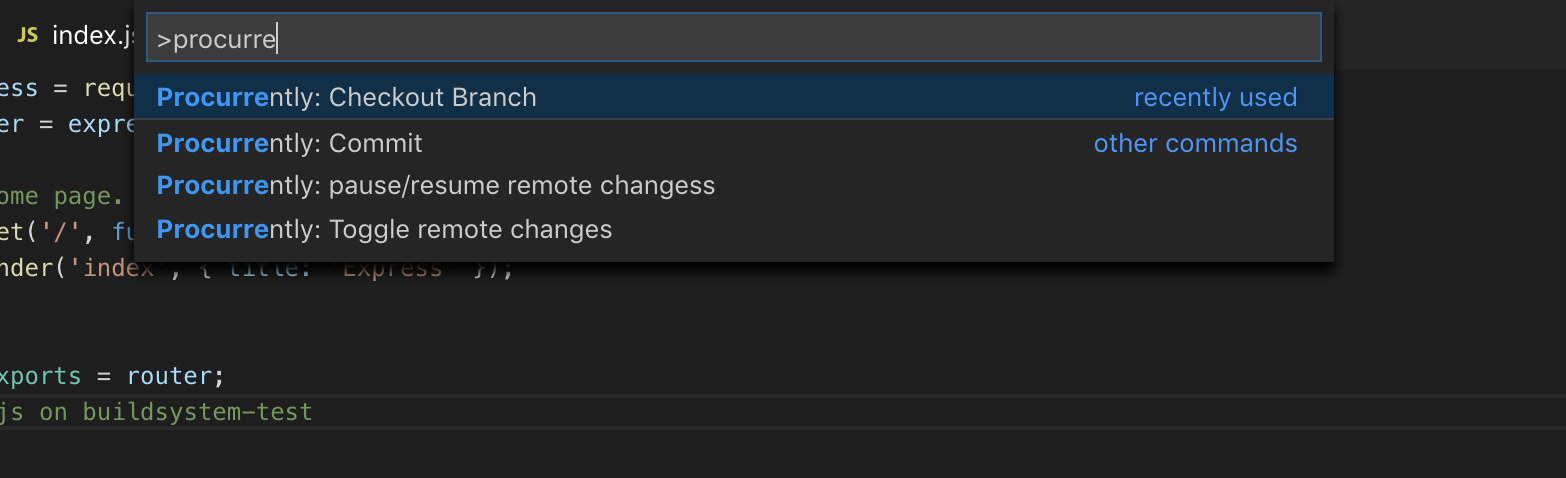
\includegraphics[width=1\linewidth]{figures/screenshots/scenarios/1checkout_branch.png}
    \caption{VS Code Command Palette Menu}
    \label{fig:1checkout_branch_palette}
\end{figure}
\begin{figure}
    \centering
    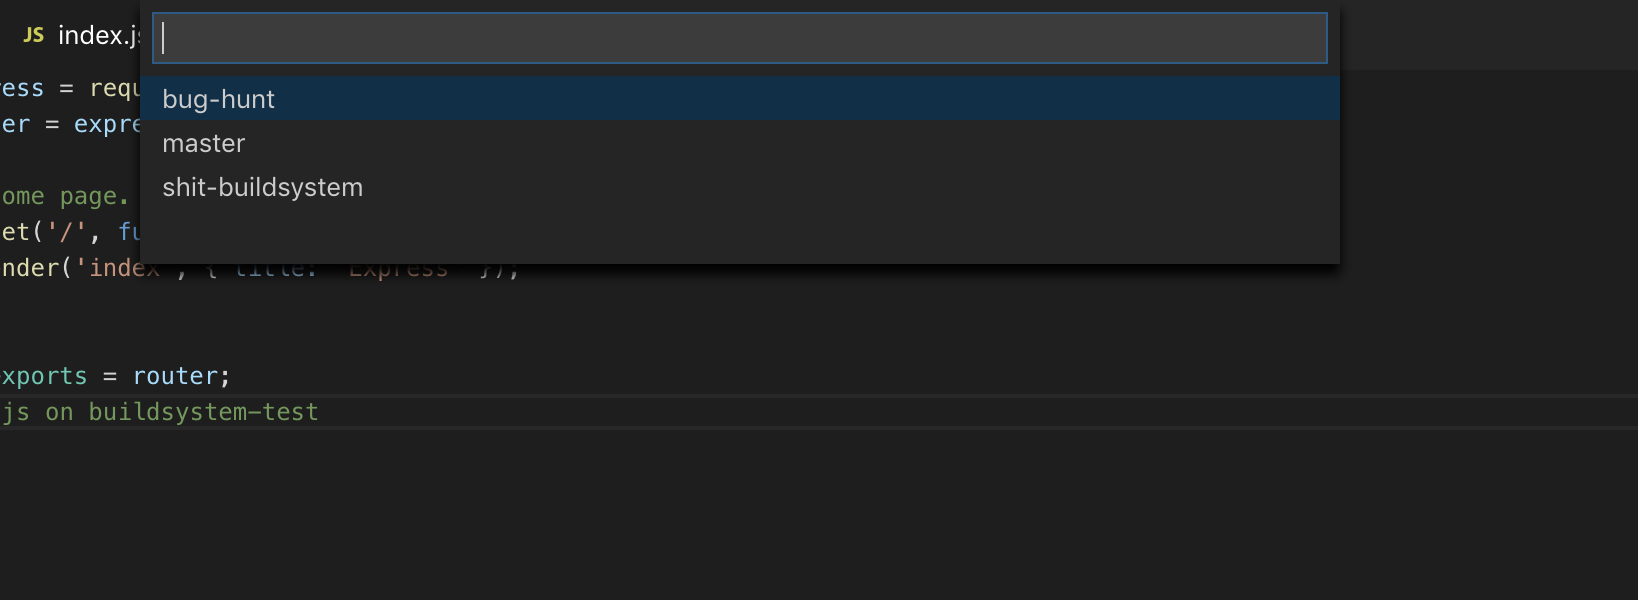
\includegraphics[width=1\linewidth]{figures/screenshots/scenarios/1checkout_bughunt.png}
    \caption{Select Branch}
    \label{fig:1checkout_bughunt}
\end{figure}


\begin{figure}[h]
    \centering
    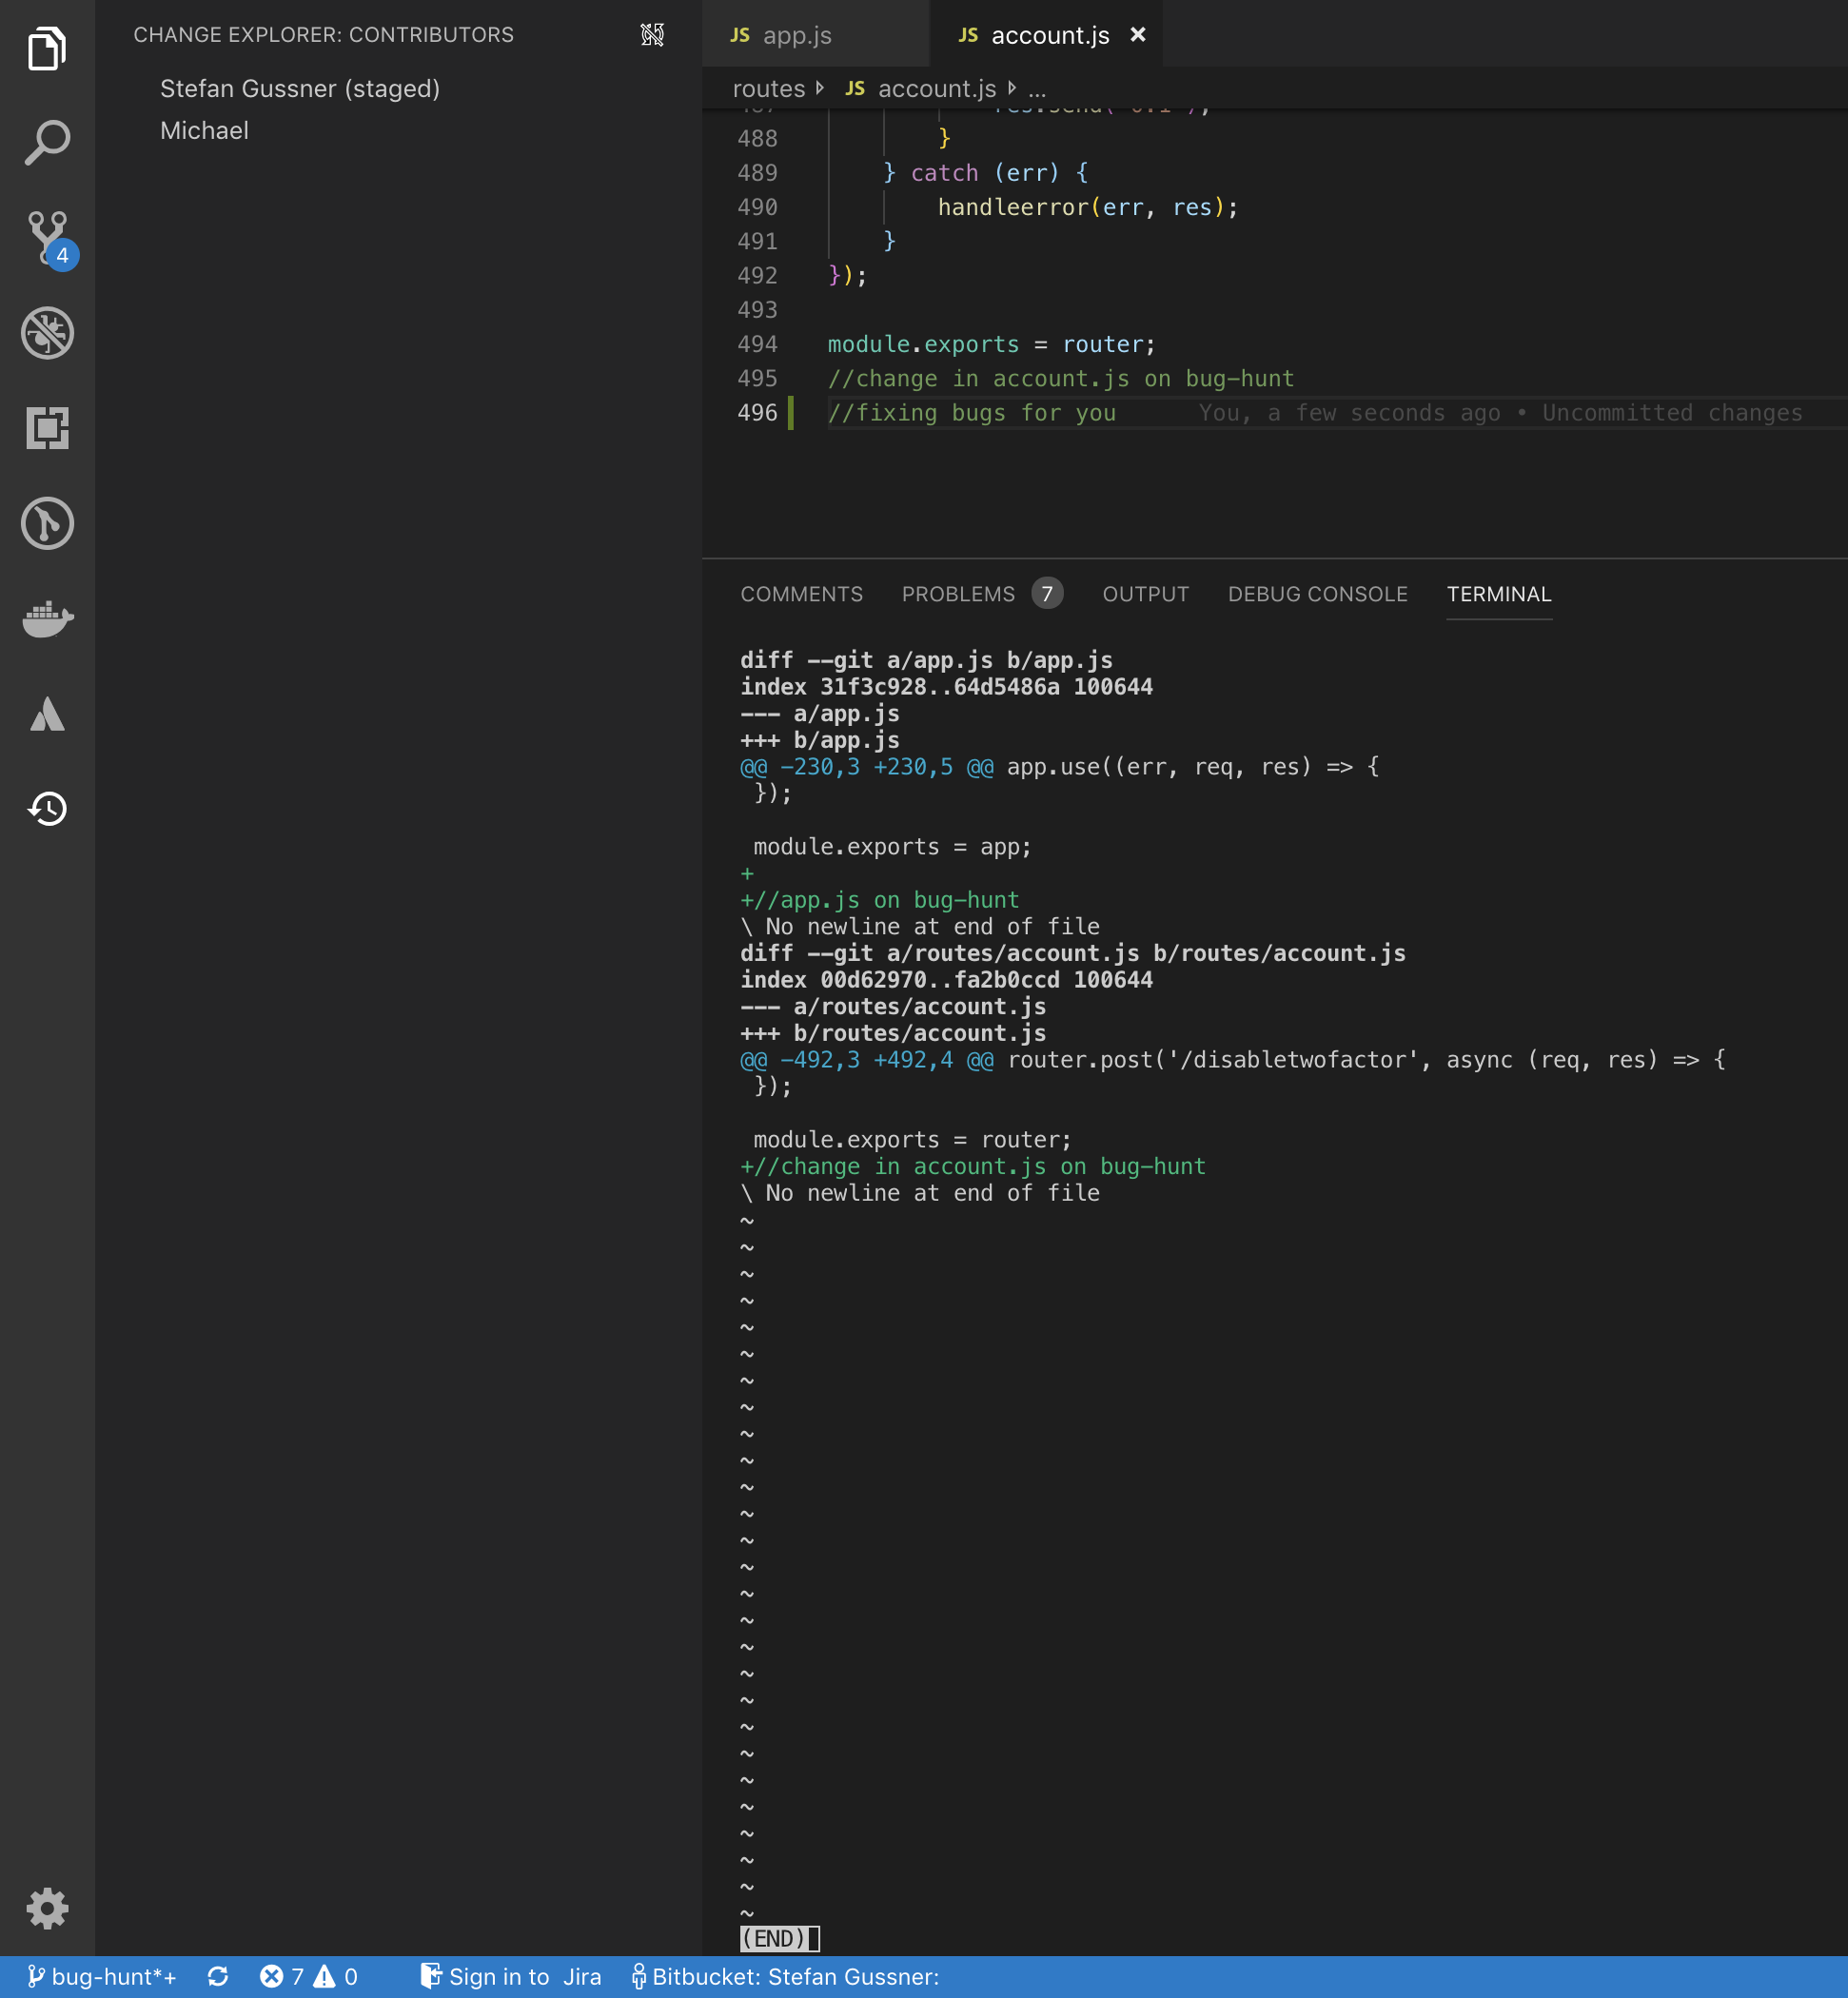
\includegraphics[width=1\textwidth]{figures/screenshots/scenarios/1staging_view.png}
    \caption{Scenario 1: account.js modified by Michael}
    \label{fig:1staging}
\end{figure}

On the computer with the Username "Michael" configured, the VS Code Command Palette was opened and the option Procurrently: Checkout Branch was selected (see \autoref{fig:1checkout_branch_palette}). From the presented options the branch "bug-hunt" was selected (see \autoref{fig:1checkout_bughunt}). All the files were closed and the files /app.js and /routes/account.js were opened. The modifications on branch "bug-hunt" were visible in the files and the changes in branch "buildsystem-test" were no longer visible. The file /routes/account.js was modified by the computer with the Username "Michael" inserting another comment (see \autoref{fig:1staging}). The changes were immediately visible on the other computer. Using the VS Code Command Palette, the computer with the Username "Michael" configured switched back to branch "buildsystem-test".

\subsection{Scenario 2}

Both computers started out on the same branch. On the computer with the username "Stefan Gussner" a comment reading "comment from stefan" was created. On the other computer a comment reading "comment from michael" was added (see \autoref{fig:2comments}). The VS Code Command Palette was used to execute the Procurrently: Toggle remote changes option (see \autoref{fig:2togglechanges}). After that, all remote changes were removed from the file and only local changes were left (See \autoref{fig:2onlylocalchanges}). Later the Command Palette was used again to execute the Procurrently: Toggle remote changes command again to display the remote changes again.

\begin{figure}
    \centering
    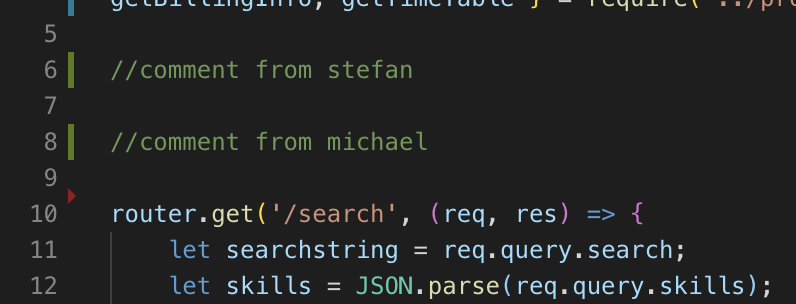
\includegraphics[width=1\textwidth]{figures/screenshots/scenarios/2comments.png}
    \caption{Scenario 2 - Comments Added by Both Collaborators}
    \label{fig:2comments}
\end{figure}
\begin{figure}
    \centering
    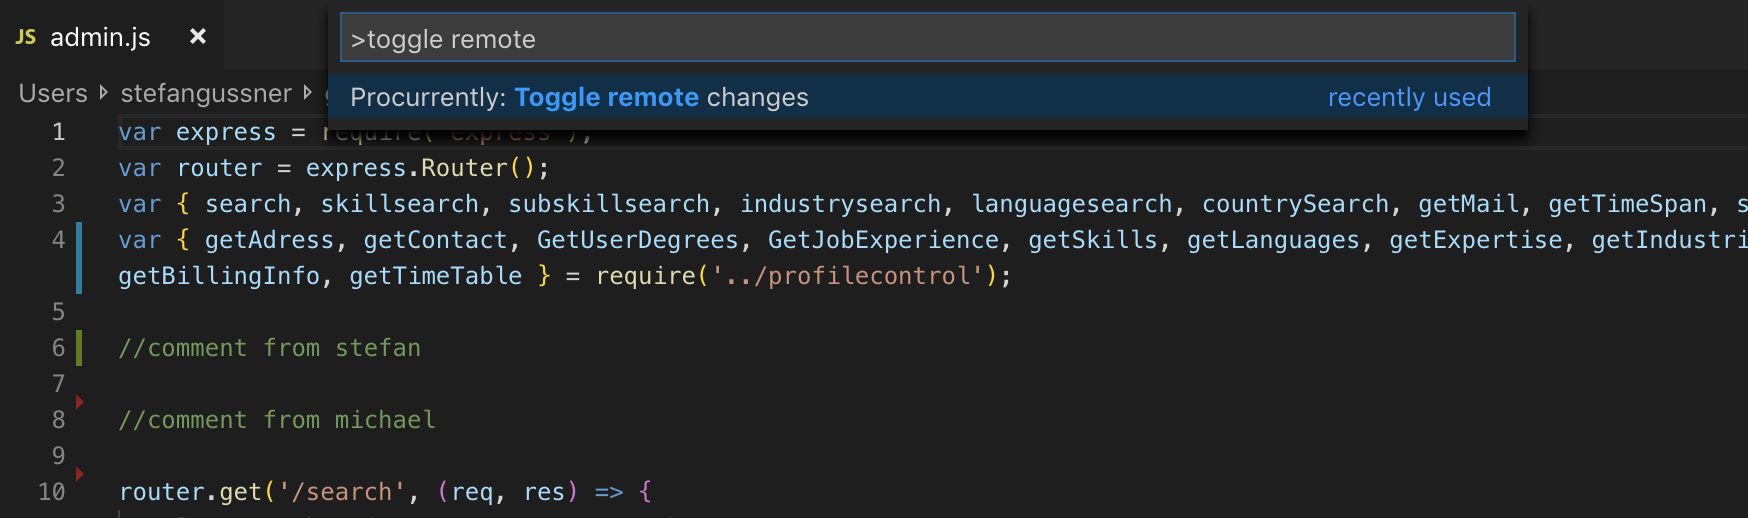
\includegraphics[width=1\linewidth]{figures/screenshots/scenarios/2togglechanges.png}
    \caption{Scenario 2 - VS Code Command Palette Menu Toggle Changes}
    \label{fig:2togglechanges}
\end{figure}

\begin{figure}[hb]
    \centering
    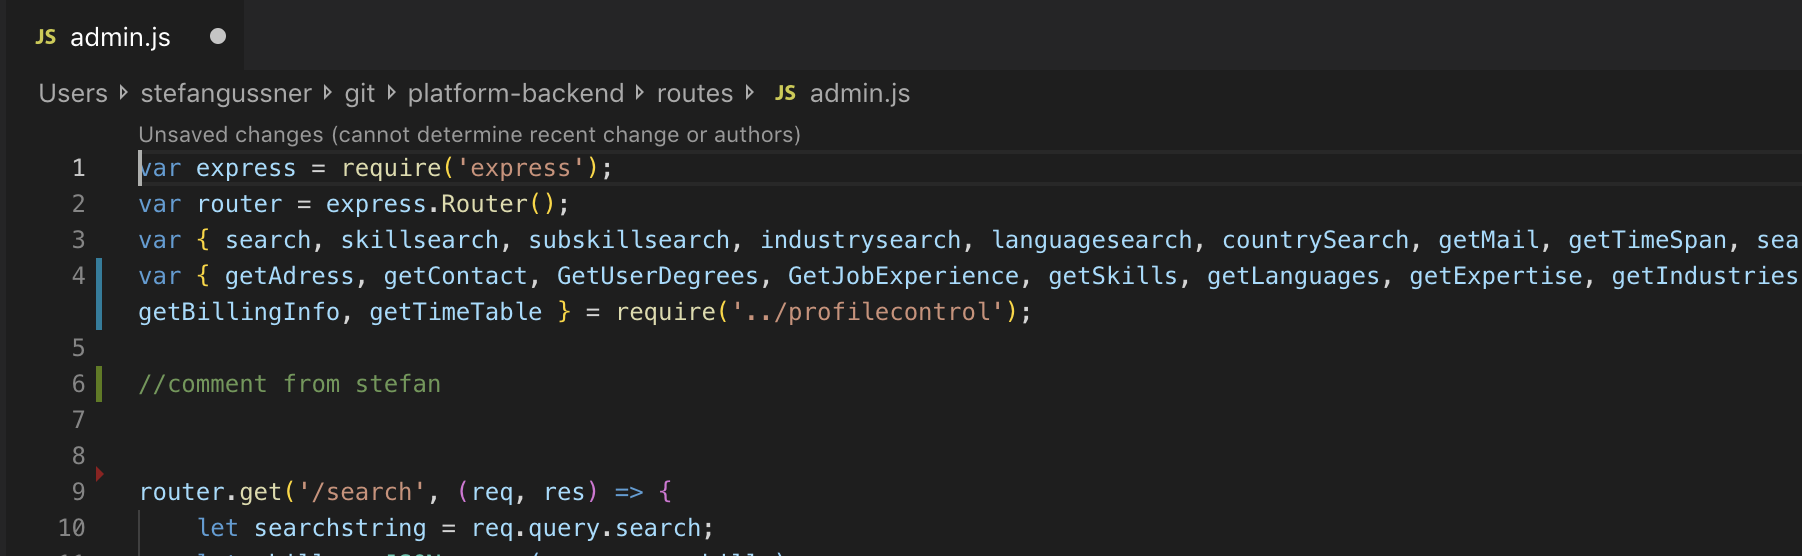
\includegraphics[width=1\textwidth]{figures/screenshots/scenarios/2onlylocalchanges.png}
	\caption{Scenario2: Only Local Changes Visible}
    \label{fig:2onlylocalchanges}
\end{figure}

\section{Results}
Procurrently succeeded in using information provided by Git to provide branch based real time document synchronization. Only changes on the same branch are displayed to other users.

Changes to all documents in Git projects are shared with other peers (note that this is not the entire project structure as described in Limitations).

Changes can be staged by author. This provides accountability and clarity about changes. \autoref{fig:stagebyauthor} shows staging a change by author using the Tree View panel. 

\begin{figure}[hb]
    \centering
    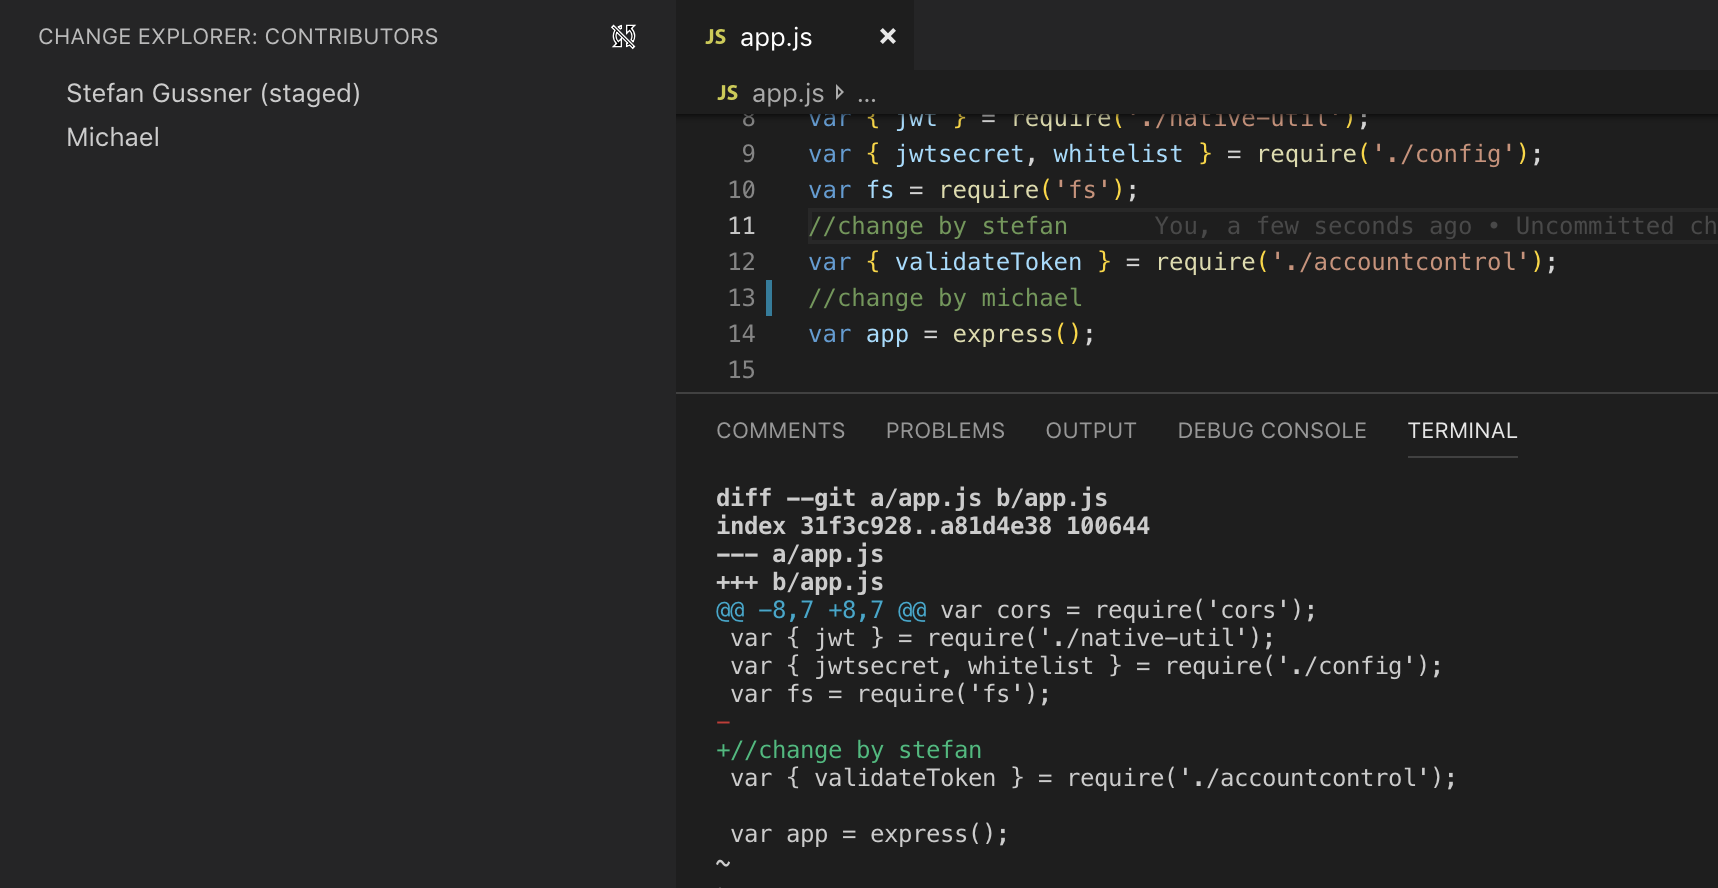
\includegraphics[width=150mm]{figures/screenshots/stage-by-author.png}
	\caption{Staging Changes by Author}
    \label{fig:stagebyauthor}
\end{figure}

Files defined to be ignored by Git are also ignored by Procurrently. This prevents accidentally publishing classified information and conflicts introduced by generated files. 

\subsection{Other Solutions}
Procurrently runs on the client and to some extent even works offline. Although some of the Tools described in \autoref{sec:stateoftheart} are client-side applications/extensions none of them provide support working offline. Having data available on the client at all times provides a performance advantage for Procurrently because when changesets have to be computed for displaying/hiding remote changes or branches are switched all the necessary data is already in memory on the device and is therefore very fast. It also enables real time collaborations in environments without a stable internet connection such as trains.

Other solutions do not consider the version control system when providing real time changes. This limits their usability in corporate environments. Procurrently is a tool for Git based environments and their use-cases in corporate environments. 

\subsection{Testing Procurrently in the Real-World}

Procurrently was tested in a real-world development environment with 2 users for 5 hours. After a short introduction to the new Git checkout procedure the tool did not cause friction for the users. During the test situations similar to \autoref{sec:scenario1} were encountered multiple times. Procurrently was working as expected and aided the problem solution by providing fast context switching without the overhead of synchronizing changes via Git.

\section{Limitations}

Compared to other current solutions, Procurrently is unable to track files that do not exist in the last Git commit because the base version of a file is derived from the latest Git commit. This behaviour is necessary because some VS Code extensions create temporary files that do not get persisted to the filesystem but fire change events. Not ignoring these files would force developers to extend their .gitignore configuration and interfere with Procurrentlys goal of not requiring extra configuration by the developer.

Procurrently is not secure. Anyone on the network can modify files in the repository. Also, all the traffic is unencrypted and can therefore be read by anyone on the network. This might not be a problem for open source projects as well as people working in corporate network environments.

The staging view does not differentiate between different branches so all collaborators across all Git repositories and branches are presented as changes to be staged instead of filtering by collaborators who changed the current working context.

Due to the possible inconsistencies introduced by the asynchronous VS Code applyEdit API function and the workaround described in \autoref{subsec:concurrentchanges} processing huge change sets is noticeably slow. This is most obvious when processing multi cursor changes with more than 20 cursors at once.

Because the networking layer does not support UDP hole punching \cite{10.1007/978-3-642-20798-3_1} or similar techniques, communication between peers only works when clients are in the same local network.

Branch switching and committing changes sometimes have to be done through custom commands in VS Code instead of having the flexibility of doing those tasks using the command line and potentially using other programs or scripts to call those functions.

Procurrently enables switching branches while the current branch has been modified and the changes would be overwritten by Git. But this feature only works when using the custom VS Code command "Procurrently: Checkout Branch".

Procurrentlys function to commit changes by author only works properly if using the custom VS Code command "Procurrently: Commit". Otherwise non committed changes will be lost after the commit because the changes are tied to the commit hash.

If there is no overlap between people working on a project, information about concurrent edits cannot be exchanged between peers.
One possible solution might be to host a Procurrently nodes in the Cloud. As described in \cite{6188603}, Cloud hosted nodes could be for Procurrently what GitHub is to Git. 
Peer to peer technology has been used to improve the Cloud before. \cite{Ranjan2013}, \cite{Ranjan2010}, \cite{Babaoglu:2012:DIP:2245276.2245357}. Cloud technology can be used to improve peer to peer software. This concept is used in the experimental Beaker Browser\footnote{https://beakerbrowser.com/docs/how-beaker-works/peer-to-peer-websites\#keeping-a-peer-to-peer-website-online}
\makeatletter\ifthesis@masterthesis
%%%%%%%%%%%%%%%%%%%%%%%%%%%%%%%%%%%%%%%%%%%%%%%%%%%%%%%%%%%%%%%%%%%%%%%%
\chapter{Diskussion}
\label{sec:discussion}
%%%%%%%%%%%%%%%%%%%%%%%%%%%%%%%%%%%%%%%%%%%%%%%%%%%%%%%%%%%%%%%%%%%%%%%%

Den akademischen Wert der Arbeit hervorheben, Vergleich mit verwandten Arbeiten: In welchem Verhältnis stehen die Ergebnisse der Diplomarbeit zu den Ergebnissen anderer Studien? Wo gibt es Unterschiede, wo Gemeinsamkeiten? Warum?

Diskussion offener Punkte, Darstellen der Stärken und Schwächen der vorliegenden Ergebnisse.
\fi\makeatother
\chapter{Conclusions}

Procurrently demonstrates an approach to real-time collaboration compatible with traditional workflows based on Git with opportunistic peer to peer communication. 

Developers do not have to think about the extension. It is possible to disable or pause remote changes. 

Developers can easily jump between branches without the need to commit work before doing so. This improves upon VCS use-cases such as helping a colleague with a problem without having to commit, push and pull changes first. 

In contrast to other real-time collaboration solutions, accountability for changes is not lost when committing to a Git repository by staging changes by author.

\section{Future Research}

The network layer of Procurrently is implemented in a very simplistic way.
Possible next research steps for more efficient network usage could be:

\begin{itemize}
    \item Providing real-time updates only to peers on the same branch and batching and bundling updates for other peers
    \item Use 5G D2D communication for the network transport for peer to peer communication \cite{TehraniUysalYanikomeroglu:2014:Device-to-devicecommunicationin5G}
    \item Encrypt traffic and authenticate collaborators
\end{itemize}

Establishing an initial shared state might be possible with local changes present instead of doing a Git reset. This might require user interaction to resolve conflicts using 1-way merges or manually changing the file contents. \cite{7070484}

Furthermore it is possible that a system like Procurrently could reduce friction in establishing group awareness by enabling group coding sessions over long distances instead of just relying on mailing lists and chats as described in \cite{Gutwin:2004:GAD:1031607.1031621} and would make it easier to know, "whom to contact" \cite{795103}, \cite{Gutwin:2004:GAD:1031607.1031621}.

As speed in Continuous Integration systems is crucial: "The dominant technical factors which explain Travis abandonment are \textbf{Build duration} and Language" \cite{8595199}, Procurrently could also find use-cases in Continuous Integration augmenting common workflows based on Git. 
Current workflows react to commits as described:

\blockquote[{\cite{8695332}}]{
    \begin{itemize}
        \item Developers builds and pushes code to Github
        \item Github will use a webhook to notify Jenkins of the recent change
        \item Jenkins will pull the Github repository, including the Dock-erfile describing the image along with the application
        \item Jenkins will then build the Docker image of that application on the Jenkins slave node
        \item Jenkins will run the Docker container on the slave node and will execute the appropriate tests
        \item If the tests are successful, the docker image is then pushed to the Docker Hub with the appropriate version number
    \end{itemize}
}

Additionally, to listing to pushes on GitHub, builds could be triggered when any developer changes a file in Procurrently, and the results of the test results could be displayed within the editor as soon as the tests have run. This could reduce feedback delay of Continuous Integration systems.

% insert bibliography and such stuff
\BackMatter

\cleardoublepage
\appendix

%%%%%%%%%%%%%%%%%%%%%%%%%%%%%%%%%%%%%%%%%%%%%%%%%%%%%%%%%%%%%%%%%%%%%%%%
\chapter{\appendixlabel}
%%%%%%%%%%%%%%%%%%%%%%%%%%%%%%%%%%%%%%%%%%%%%%%%%%%%%%%%%%%%%%%%%%%%%%%%

\whichlanguage{
Listings, data models, forms, \dots
}{
Quellcode, Datenmodell, Fragebögen, \dots
}

\end{document}
